\documentclass{article}
\usepackage{tikz}
\usepackage{pgfplots}
\pgfplotsset{compat=1.17}
\usetikzlibrary{shapes.geometric, arrows, positioning}
\usetikzlibrary{decorations.pathreplacing, shapes.geometric, arrows, positioning}
\definecolor{maroon}{rgb}{0.5, 0, 0}
\definecolor{darkblue}{rgb}{0.0, 0.0, 0.55}
\definecolor{pblue}{HTML}{2980FF}
\definecolor{plightred}{HTML}{FF7676}
\definecolor{pdarkred}{HTML}{FF000D}
\usepackage{amsmath}
\usepackage{fontawesome}
\tikzstyle{process} = [rectangle, rounded corners, minimum width=2.5cm, minimum height=1cm, text centered, draw=black, fill=blue!20]
\tikzstyle{process1} = [rectangle, rounded corners, minimum width=0.8cm, minimum height=0.8cm, text centered, draw=black, fill=darkblue!50]
\tikzstyle{process2} = [rectangle, rounded corners, minimum width=0.8cm, minimum height=0.8cm, text centered, draw=black, fill=maroon!50]
\tikzstyle{arrow} = [thick,->,>=stealth]
% Optional math commands from https://github.com/goodfeli/dlbook_notation.

\usepackage{url}
\usepackage{booktabs}
\usepackage{subcaption}
\usepackage{multirow}

\usepackage{arxiv}

\usepackage[utf8]{inputenc} % allow utf-8 input
\usepackage[T1]{fontenc}    % use 8-bit T1 fonts
\usepackage{hyperref}       % hyperlinks
\usepackage{url}            % simple URL typesetting
\usepackage{booktabs}       % professional-quality tables
\usepackage{amsfonts}       % blackboard math symbols
\usepackage{nicefrac}       % compact symbols for 1/2, etc.
\usepackage{microtype}      % microtypography
\usepackage{lipsum}		% Can be removed after putting your text content
\usepackage{graphicx}
\usepackage[numbers]{natbib}
\usepackage{doi}



\title{Accelerated Gradient-based Design Optimization Via Differentiable Physics-Informed Neural Operator: \newline A Composites Autoclave Processing Case Study}

\newcommand*\samethanks[1][\value{footnote}]{\footnotemark[#1]}
%\date{September 9, 1985}	% Here you can change the date presented in the paper title
%\date{} 					% Or removing it

\author{{\hspace{1mm}Janak M. Patel}\thanks{Corresponding author.} \\
        Applied Research, Quantiphi\\
        Marlborough, MA 01752, USA\\
	\texttt{janak.patel@quantiphi.com} \\
	%% examples of more authors
	\And
	{\hspace{1mm}Milad Ramezankhani}\\
	Applied Research, Quantiphi\\
        Marlborough, MA 01752, USA\\
	\texttt{milad.ramezankhani@quantiphi.com} \\
        \And
	{\hspace{1mm}Anirudh Deodhar} \\
	Applied Research, Quantiphi\\
        Marlborough, MA 01752, USA\\
	\texttt{anirudh.deodhar@quantiphi.com} \\
        \And
	{\hspace{1mm}Dagnachew Birru} \\
	Applied Research, Quantiphi\\
        Marlborough, MA 01752, USA\\
	\texttt{dagnachew.birru@quantiphi.com} \\
	%% \AND
	%% Coauthor \\
	%% Affiliation \\
	%% Address \\
	%% \texttt{email} \\
	%% \And
	%% Coauthor \\
	%% Affiliation \\
	%% Address \\
	%% \texttt{email} \\
	%% \And
	%% Coauthor \\
	%% Affiliation \\
	%% Address \\
	%% \texttt{email} \\
}

% Uncomment to remove the date
%\date{}

% Uncomment to override  the `A preprint' in the header
%\renewcommand{\headeright}{Technical Report}
%\renewcommand{\undertitle}{Technical Report}
\renewcommand{\shorttitle}{Accelerated Gradient-based Design Optimization Via Physics Informed Neural Operator}

%%% Add PDF metadata to help others organize their library
%%% Once the PDF is generated, you can check the metadata with
%%% $ pdfinfo template.pdf
\hypersetup{
pdftitle={A template for the arxiv style},
pdfsubject={q-bio.NC, q-bio.QM},
pdfauthor={David S.~Hippocampus, Elias D.~Striatum},
pdfkeywords={First keyword, Second keyword, More},
}

\begin{document}
\maketitle

\begin{abstract}
Simulation and optimization are crucial for advancing the engineering design of complex systems and processes. Traditional optimization methods require substantial computational time and effort due to their reliance on resource-intensive simulations, such as finite element analysis, and the complexity of rigorous optimization algorithms. Data-agnostic AI-based surrogate models, such as Physics-Informed Neural Operators (PINOs), offer a promising alternative to these conventional simulations, providing drastically reduced inference time, unparalleled data efficiency, and zero-shot super-resolution capability. However, the predictive accuracy of these models is often constrained to small, low-dimensional design spaces or systems with relatively simple dynamics. To address this, we introduce a novel Physics-Informed DeepONet (PIDON) architecture, which extends the capabilities of conventional neural operators to effectively model the nonlinear behavior of complex engineering systems across high-dimensional design spaces and a wide range of dynamic design configurations. This new architecture outperforms existing state-of-the-art models, enabling better predictions across broader design spaces. Leveraging PIDON's differentiability, we integrate a gradient-based optimization approach using the Adam optimizer to efficiently determine optimal design variables. This forms an end-to-end gradient-based optimization framework that accelerates the design process while enhancing scalability and efficiency. We demonstrate the effectiveness of this framework in the optimization of aerospace-grade composites curing processes achieving a \(3 \times\) speedup in obtaining optimal design variables compared to gradient-free methods. Beyond composites processing, the proposed model has the potential to be used as a scalable and efficient optimization tool for broader applications in advanced engineering and digital twin systems.
\end{abstract}


% keywords can be removed
\keywords{Neural operator \and Physics-informed DeepONet \and Gradient-based optimization \and Composite materials \and Curing processes}
\section{Introduction}
Simulation and optimization play a pivotal role in modern engineering, serving as essential tools for analyzing, designing, and enhancing complex systems and processes. Engineers leverage simulation models to explore design spaces, evaluate performance, and guide decision-making through optimization. Traditionally, numerical simulation methods, such as finite element analysis, have been widely used in combination with optimization algorithms to determine optimal design variables \cite{struzziero2017multi,dolkun2018optimization,tang2022multi}. However, these methods are computationally expensive and time-intensive, making them less practical for real-time or iterative-based design processes \cite{ZIMMERLING2022110423}. To address these challenges, machine learning-based surrogate models have been developed as alternatives to reduce computational costs \cite{pfrommer2018optimisation, tifkitsis2018stochastic,yuan2021multi}. Once trained, these models provide fast predictions, enabling near real-time optimization. However, surrogate models often require large datasets for training, which is prohibitive in many industrial scenarios with data scarcity, resulting in unreliable or physically implausible predictions.

Recently, Physics-Informed Neural Networks (PINNs) are introduced \cite{raissi2019physics}, which incorporate governing partial differential equations (PDEs) into the loss function of a neural network. This allows the model to learn directly from the underlying physics, combining the strengths of numerical methods with machine learning-based surrogate modeling. While PINNs offer a promising alternative for solving PDEs without requiring labeled data, they are typically trained on fixed initial and boundary conditions (ICs/BCs) \cite{wang2022mosaic}. This limitation makes them less practical for iterative design optimization tasks, where system configurations (e.g., different BCs) frequently change. In contrast, neural operators such as DeepONet \cite{lu2019deeponet} and Fourier neural operator (FNO) \cite{li2020fourier}, which directly map infinite-dimensional input-output function spaces on bounded domains, are capable of learning a family of PDEs rather than a single instance \cite{boulle2023mathematical,kovachki2023neural}. Inspired by PINNs, Physics-Informed Neural Operators (PINOs) extend this capability by incorporating physics constraints into the loss function, allowing them to solve PDE families without relying on data \cite{wang2021learning,goswami2023physics}. Unlike PINNs, PINOs enable real-time predictions under varying conditions, making them ideal for design optimization. Despite the advantages of PINOs in capturing system dynamics under varying conditions, existing architectures may struggle with high-dimensional and large design spaces for real-world engineering problems. Additionally, traditional gradient-free optimization methods, such as Particle Swarm Optimization (PSO) \cite{pyswarmsJOSS2018} and Genetic Algorithms (GA) \cite{solgi_geneticalgorithm}, often require a large number of function evaluations, making them computationally expensive and inefficient for high-dimensional optimization \cite{allen2022physical}. 

To address these challenges, we propose an accelerated gradient-based optimization framework tailored for advanced engineering design. Specifically, Our work focuses on composite materials processing, where achieving an optimal cure cycle is critical for ensuring material quality. Composite materials are extensively used in aerospace, automotive, and marine industries due to their high strength, durability, and lightweight properties \cite{li2020cure}. These materials undergo a polymerization process governed by a temperature and pressure cycle known as the cure cycle \cite{strong2008fundamentals}. The cure cycle must be optimized to ensure uniform resin curing while minimizing residual stress and deformation \cite{hubert2001cure}. Since changes in part geometry or material properties often require adjustments to the cure cycle, optimization becomes essential for ensuring high-quality and reliable composites.

Numerous studies have utilized PINO models to simulate the thermochemical evolution of composites during autoclave curing. For instance, a Physics-guided Neural Operator is developed for composite manufacturing \cite{chen2023physics}. Similarly, physics-informed FNO was applied to analyze the curing process of carbon-fiber composites \cite{meng2023novel}. Furthermore, a Physics-Informed DeepONet, enhanced with advanced features such as nonlinear decoders and curriculum learning is developed for modeling complex thermochemical processes \cite{ramezankhani2025advanced}. However, the predictive performance of these models remains satisfactory only when applied to single-variable designs, limited design spaces, or systems with low behavioral complexity. This limitation may arise from the inherent constraints of the original neural operator architecture in handling nonlinear and stiff problems, as well as complex physics-informed loss landscape \cite{krishnapriyan2021characterizing} and neural network's spectral bias \cite{rahaman2019spectral}. To address these challenges and ensure that the developed surrogate model remains accurate when exposed to high-dimensional and large design spaces for optimization tasks, we propose an advanced Physics Informed DeepONet (PIDON) architecture. In particular, it incorporates domain decomposition with separate DeepONets allocated to each temporal subdomain, as well as input coordinate normalization to mitigate spectral bias \cite{moseley2023finite}. Furthermore, each subdomain is equipped with a nonlinear decoder to better capture the complex dynamics of the PDE. The proposed PIDON model serves as an efficient and accurate surrogate for inverse design, enabling near real-time spatiotemporal predictions for given design conditions. This capability enhances design space exploration and accelerates the identification of optimal design variables to achieve desired material properties. Leveraging the differentiability of PIDON \cite{li2024physics}, we utilize a gradient-based optimization technique, which significantly reduces the number of function evaluations and improves scalability for larger design spaces compared to gradient-free methods \cite{allen2022physical}. The Adam optimizer \cite{kingma2014adam} is used to obtain the optimal design variables. We benchmark this framework against gradient-free methods, including PSO and GA. The main contributions of this paper are summarized as:
% \begin{itemize}  
%     \item \textbf{AI-driven Accelerated Design Optimization framework:} Development of an end-to-end framework for accelerated AI-driven design optimization of the curing process for composite materials
%     \item \textbf{Novel PIDON Architecture:} Development of PIDON model with domain decomposition, separate input normalization for each subdomain and a nonlinear decoder
%     \item \textbf{Gradient-Based Optimization:} Integration of the Adam optimizer with the differentiable PIDON model, achieving efficient and scalable optimization compared to traditional gradient-free methods
% \end{itemize}  
\begin{itemize}  
    \item Design and implement an improved PIDON model for composites manufacturing, enabling an accurate and accelerated exploration of high-dimensional and large design spaces.
    \item Develop an end-to-end AI-driven design optimization framework enabling \(3\times\) speedup over conventional gradient-free approaches.
\end{itemize}  
\section{Methodology}
\subsection{Composites autoclave processing}
\label{composites}
The autoclave processing in the manufacture of composites involves placing resin-impregnated fibers and a tool into an autoclave, where the system undergoes a cure cycle to achieve the desired material properties, as illustrated in Figure \ref{fig:system}.a. The temperature distribution within the part ($T_c$) and tooling ($T_t$), along with the progression of the resin's degree of cure (DOC), are critical state variables in composites systems. The thermochemical behavior of a 1D composite-tool system in an autoclave is described by the following one-dimensional anisotropic heat conduction equation:
\begin{equation}
\begin{aligned}
\frac{\partial T_t}{\partial t} &= a_t \frac{\partial^2 T_t}{\partial z^2}, \quad z \in [0, L_t] \\
\frac{\partial T_c}{\partial t} &= a_c \frac{\partial^2 T_c}{\partial z^2} + b_c \frac{\partial \alpha}{\partial t}, \quad z \in [L_t, L_c]
\end{aligned}
\end{equation}
Here, $T$ is the temperature, $\alpha$ is DOC, $L_c$ is the material length, $L_t$ is the tool length, and $t$ and $z$ are the spatiotemporal coordinates. The subscripts $t$, $c$, and $r$ represent the tool, composite part, and resin, respectively. The parameter $a$ denotes the thermal diffusivity, and $b$ represents the heat generation coefficient. For the curing process of a composite system with thermoset resin, the cure rate is governed by the resin's cure kinetics, which are typically represented by an ordinary differential equation. For the AS4/8552 epoxy resin system, it can be expressed as follows\citep{hubert2001cure}:
\begin{equation}
\frac{\partial \alpha}{\partial t} = A \exp\left(-\frac{\Delta E}{RT}\right) \frac{1}{1 + \exp\left(C(\alpha - (C_0 + C_T T))\right)} \alpha^m (1 - \alpha)^n
\end{equation}
where, $\Delta E$ represents the activation energy, $R$ is the gas constant, and $C_0$, $C_T$, $m$, $n$, and $A$ are experimentally determined constants and parameter. The values used for this study can be found in \citep{johnston1997integrated}.
Considering the convective heat transfer between the autoclave air $T_a$ and the composite system, the boundary conditions are governed by:
\begin{equation}
\begin{aligned}
(T_a - T_c \big|_{z=L_c}) &= \frac{k_c}{h_{\text{top}}} \frac{\partial T_c}{\partial z} \Bigg|_{z=L_c} \\
(T_t \big|_{z=0} - T_a) &= \frac{k_t}{h_{\text{bot}}} \frac{\partial T_t}{\partial z} \Bigg|_{z=0}
\end{aligned}
\end{equation}
Here, $h_{\text{top}}$ and $h_{\text{bot}}$ are the convective heat transfer coefficients (HTCs) on the top and bottom surfaces of the composite-tool system, respectively, while $k_c$ and $k_t$ represent the thermal conductivity of the composite and tool, respectively. The initial temperature of the part is typically assumed to be uniform throughout. For this study, we assume an initial temperature of 20°C. The initial DOC is assumed to be either zero or a very small value for an uncured part and in this study, is set to 0.05. The part thickness is fixed for this study, while the tool thickness is included as one of the design variables. To manage inconsistencies in the total system length and interface location resulting from variations in tool thickness, local coordinates are introduced, following the approach outlined by \citep{ramezankhani2025advanced}.

A typical two-hold cure cycle consists of two distinct stages where the air temperature is held constant at specific levels for predetermined durations. This approach enables a controlled progression of the curing process, allowing optimal material properties to be achieved while minimizing potential issues such as under-curing or over-curing \citep{fabris2018framework}. The cure cycle is defined using six key design variables: heating rates \(r_1\) and \(r_2\) (the rate at which the air temperature inside the autoclave increases), hold durations \(hd_1\) and \(hd_2\) (the time periods for which the temperature is maintained constant at the respective hold temperatures) and hold temperatures \(ht_1\) and \(ht_2\) (the target temperatures held during the first and second stages).
\begin{figure*}[t]  
    \centering
    \includegraphics[width=1\textwidth]{paper_arch_plot_v2.pdf} 
    \caption{a) Schematic representation of the composite-tool system inside an autoclave, including local coordinates $x_1$ and $x_2$ (adopted from \cite{ramezankhani2025advanced}). b) Architecture of the proposed sub-PIDON model for predicting part temperature \(G^{T_c}\). The same architecture is utilized for other output variables, including DOC \(G^{\alpha}\) and tool temperature \(G^{T_t}\). c) Illustration of the proposed PIDON framework with a nonlinear decoder and domain decomposition, designed for thermochemical analysis during the composite curing process.}     % Caption for the figure
    \label{fig:system}                             % Label for referencing the figure
\end{figure*}
\subsection{Differentiable Simulator: Physics Informed DeepONet} 
The architecture of DeepONet has two primary components: a branch and a trunk network \citep{lu2019deeponet}. The branch network takes as input the sensor point evaluations $u$ $=$ $[u(x_1), u(x_2)$,$\dots, u(x_m)]$  and generates a feature representation $b$ $=$ $[b_1, b_2, \dots, b_q]^T \in \mathbb{R}^q$ as its output. Similarly, the trunk network encodes the spatiotemporal coordinates of the PDE system \( y \) into a feature embedding \( t = [t_1, t_2, \dots, t_q]^T \in \mathbb{R}^q \), with the same dimensionality as the output of the branch network. The outputs from these networks are combined using an element-wise product operation, followed by summation, to produce the final output of the DeepONet:
\begin{equation}
G_\theta(u)(y) = \sum_{k=1}^{q} b_k t_k + b_0
\end{equation}
Data-driven DeepONet often requires large amounts of training data, which can be difficult to access in many real-world engineering applications. The physics-informed variant of DeepONet, namely PIDON, integrates governing equations directly into the loss function as regularizers, eliminating DeepONet's reliance on data. Specifically, the output of the PIDON is constrained to satisfy the governing equations by minimizing the loss function:
\begin{equation}
\mathcal{L}(\theta) = \mathcal{L}_{IC}(\theta) + \mathcal{L}_{BC}(\theta) + \mathcal{L}_{physics}(\theta)
\end{equation}
where $\mathcal{L}_{IC}$, $\mathcal{L}_{BC}$, and $\mathcal{L}_{physics}$ represent the initial condition (IC) loss, boundary condition (BC) loss, and physics loss, respectively. Assuming a constant initial condition and a Robin boundary condition in the introduced composites case study, \(\mathcal{L}_{IC}\) and \(\mathcal{L}_{BC}\) can be expressed as:
\begin{equation}
\mathcal{L}_{IC}(\theta) = \frac{1}{NQ_{ic}} \sum_{i=1}^{N} \sum_{j=1}^{Q_{ic}} \left| G_{\theta}(u^{(i)})(y^{(i)}_j) - s^{(i)}(y^{(i)}_j) \right|^2
\end{equation}
\begin{equation}
\mathcal{L}_{BC}(\theta) = \frac{1}{NQ_{bc}} \sum_{i=1}^{N} \sum_{j=1}^{Q_{bc}} \left| \alpha G_{\theta}(u^{(i)})(y^{(i)}_j) + \beta \nabla G_{\theta}(u^{(i)})(y^{(i)}_j) - \gamma \right|^2
\end{equation}

Here, \(u^{(i)}\) denotes the \(i\)-th input function, \(y_j^{(i)}\) represents the \(j\)-th collocation point , and \(G_\theta\) is the output of the PIDON. The term \(s^{(i)}(y_j^{(i)})\) corresponds to the solution of the partial differential equation (PDE) at \(y_j^{(i)}\), conditioned on the \(i\)-th input function. For the Robin boundary condition, \(\alpha\), \(\beta\), and \(\gamma\) are non-zero constants determined by the physical characteristics of the problem. The physics loss \(\mathcal{L}_{physics}\) is defined as:

\begin{equation}
\mathcal{L}_{physics}(\theta) = \frac{1}{NQ} \sum_{i=1}^{N} \sum_{j=1}^{Q} \left| \mathcal{N}(u^{(i)}(x), G_{\theta}(u^{(i)})(y^{(i)}_j)) \right|^2
\end{equation}

Here, \( \mathcal{N} \) denotes the nonlinear differential operator. The parameter \( N \) represents the number of distinct input function combinations sampled from the design space, whereas \( Q \) indicates the number of residual points employed to enforce the physical constraints. These \( N \) and \( Q \) are hyperparameters that can be tuned to balance the model's performance and computational efficiency. DeepONet is considered differentiable because it is a neural network-based approach that learns a solution operator, and a neural network is a differentiable function \cite{lu2019deeponet}.

\subsubsection{Proposed Architecture of PIDON}
We introduce a novel PIDON architecture designed to model the highly nonlinear dynamics of composite-tool systems during the curing process. The key components of the framework are outlined below. 

\textbf{Network architecture}.  This architecture incorporates a branch network, a trunk network, and a nonlinear decoder, drawing inspiration from advancements in operator learning \citep{seidman2022nomad, haghighat2024deeponet, ramezankhani2025advanced}. As illustrated in Figure \ref{fig:system}.b, the branch network is designed with multi-input functionality, accommodating 9 input parameters: six cure cycle parameters (\(r_1, r_2, hd_1, hd_2, ht_1, ht_2\)), two equipment design parameters(\(h_{top}, h_{bot}\), representing the convective heat transfer coefficients on the top and bottom surfaces of the composite-tool system, respectively), and one tool design parameter (tool thickness, \(L_t\) ). The trunk network takes spatio-temporal coordinates \(t\) and \(z\) as inputs. Standard DeepONet architectures with linear decoders require a large output dimension for branch and trunk networks to model nonlinear systems, making them computationally expensive and ineffective in such scenarios. In this work, we incorporate a nonlinear decoder by introducing an additional neural network that takes as input the combined output of the branch and trunk networks and generates the final output of PIDON.

\textbf{Temporal domain decomposition}. The composites curing process is a time-consuming process which requires solving the corresponding PDE equations over a long temporal domain. This poses some training challenges due to spectral bias and training difficulties such as activation saturation from large input coordinates. A temporal domain decomposition strategy is proposed, where a single DeepONet is trained with initial conditions as additional input functions \cite{wang2023long}. This enables the model to independently learn solution operators for different subdomains while ensuring temporal continuity. However, inaccuracies in predicting initial conditions can introduce and propagate errors in the model predictions. Our framework improves temporal domain decomposition by employing multiple DeepONets with separate spatiotemporal input normalization for each subdomain. In particular, the temporal domain is divided into $n$ smaller temporal subdomains based on the system's physical characteristics, with each subdomain modeled by an independent DeepONet, termed \textbf{sub-PIDON} (Figure~\ref{fig:system}.c). This setup enables each sub-PIDON to accurately capture the dynamics specific to its respective subdomain while reducing errors associated with relying on a single model to represent both initial conditions and other input functions within the system. The incorporation of separate subdomain normalization alongside domain decomposition effectively mitigates spectral bias over extended temporal domains by ensuring that the solution frequency encountered within each subdomain remains low \citep{moseley2023finite}.

\textbf{Multi-output functionality}. The PIDON framework predicts three key state variables for the thermochemical evolution in the composites curing process: $T_c$,  $T_t$, and $\alpha$. Due to the system's complexity, a single DeepONet may not effectively learn all these variables. Instead, we develop three dedicated and decoupled neural operators: \(G^{T_c}\) for composite temperature, \(G^{T_t}\) for tool temperature, and \(G^{\alpha}\) for the DOC, with each DeepONet specifically designed for its respective variable while maintaining consistent architectural principles. Thus, for each subdomain (highlighted with light and dark grey in Figure~\ref{fig:system}.c), we train three sub-PIDON, each dedicated to an output variable.
\subsubsection{Training Procedure}
As depicted in Figure \ref{fig:system}.c, the proposed PIDON framework is trained sequentially across multiple temporal subdomains. The training process begins with the initialization and training of the first sub-PIDON module (\texttt{sub-PIDON 1}) using the system’s global IC across the design space (i.e., input functions). Upon completion of its training, this module generates predictions that serve as the local IC for the subsequent sub-PIDON module (\texttt{sub-PIDON 2}). In this manner, the IC for each subdomain is determined based on the predictions of the preceding sub-PIDON model, as indicated by the green arrows in Figure \ref{fig:system}.c. This iterative process continues until all sub-PIDON modules corresponding to the defined subdomains are fully trained. The subdomains are initially partitioned into segments of equal width; however, their widths are adaptively refined during training. Specifically, if the total training loss for a given subdomain fails to reach a predefined threshold, the subdomain is further subdivided into two smaller intervals, thereby simplifying the learning task for the corresponding sub-PIDON modules. This adaptive approach enables more substantial progression in regions of the time domain where nonlinearity is less pronounced, while ensuring that highly complex regions are modeled with finer resolution. As a result, the framework maintains both computational efficiency and predictive accuracy across varying levels of system complexity.
\subsection{AI-Driven Accelerated Design Optimization Framework}
We developed an AI-driven accelerated design optimization framework for composite synthesis in autoclaves, as illustrated in Figure \ref{fig:pino_framework}. This framework integrates a generalized, accurate, and computationally efficient PIDON model, serving as a differentiable simulator to optimize the curing process. By leveraging the zero-shot super-resolution capabilities of PIDON across diverse design parameters and its differentiability for gradient-based optimizers like Adam, our framework enables rapid and efficient exploration of design variables.
\subsubsection{Design Tasks}
Several studies have focused on optimizing the cure cycle for composite synthesis to achieve various objectives. For instance, one study aimed to minimize residual stress and ensure uniform curing \cite{shah2018optimal},while another focused on maximizing the DOC, controlling peak temperature, minimizing post-gelation gradients, and reducing curing time \cite{vafayan2015development}. 

This study aims to optimize the cure cycle of AS4/8552 composites by balancing mechanical performance and structural integrity through four key objectives. The first objective is achieving a desired DOC within the range $0.85 < \alpha \big|_{t=t} < 0.95$, ensuring optimal mechanical properties while avoiding brittleness \citep{rothenhausler2023interplay}. Second, minimizing DoC gradients $\frac{\partial \alpha}{\partial x} \big|_{t=t}$ is critical for reducing residual stress and shrinkage \citep{yuan2021multi}. Third, maximum part temperature (exotherm) must remain below 185 $^{\circ}\text{C}$ to prevent thermal degradation \citep{fabris2018framework}. Finally, controlling thermal lag ($\Delta T < 20\,^{\circ}\text{C}$) ensures even curing by limiting temperature differences between autoclave air and composite parts \citep{fabris2018framework}. These objectives are essential to optimize curing for performance and material integrity.
\begin{figure}[h!]
\centering
\begin{tikzpicture}[scale=0.7, transform shape]
% Create big box
\fill[gray, opacity=0.3,rounded corners=10pt] (-7.5,-5) rectangle (13.5,2.5);

% intial design box
\fill[white, opacity=0.7, rounded corners=10pt] (-7,-4) rectangle (-3,1.5);
% --- Line Plot ---
\node (plot) at (-5,0) {
\begin{tikzpicture}
    \begin{axis}[
        width=5cm, height=4cm,
        xlabel={t}, ylabel={T},
        grid=both, 
        axis lines=middle, 
        xtick=\empty, ytick=\empty,
        ymin=0, ymax=5,
        xmin=0, xmax=6,
        legend style={at={(0.5,-0.2)},anchor=north}
    ]
    % Line plot: positive ramp, horizontal, positive ramp, horizontal, negative ramp
    \addplot[thick, darkblue] coordinates {
        (0,0.1) 
        (1,2)  % Positive ramp
        (2,2)       % Horizontal line
        (3,4)       % Positive ramp
        (4,4)       % Horizontal line
        (5,0.2)      % Negative ramp
    };
    \node at (axis cs: 3, 1.4) {Cure Cycle};
    \end{axis}
\end{tikzpicture}
};

% --- Nodes ---
% Inputs to the PINO Model
\node (ht) at(-6.25,-2) [process1] {$h_{top}$};
\node (hb) at(-5,-2) [process1] {$h_{bottom}$};
\node (Lt) at(-3.75,-2) [process1] {$L_{t}$};
\node (plus) at(-5,-1.4) {$+$};

% Curly bracket around the three nodes
\draw [decorate,decoration={brace,amplitude=8pt,mirror}] 
  (ht.south west) -- (Lt.south east) node [black,midway,xshift=0.4cm]{};
\node (designtitle) at(-5,-3.3) {\textit{Tool and Equipment}};
\node (designtitle) at(-5,-3.6) {\textit{Design Variable}};
\draw[->, thick] (-3,-1.25) -- (-1,-1.25);

% PINO Model box
\fill[white, opacity=0.7 , rounded corners=10pt] (-1,-4) rectangle (3.5,1.5);
% Sub-rectangle 1 (with only the border in maroon)
\draw [rounded corners=5pt, thick, draw=plightred] (-0.5,-1.1) rectangle (1.5,1.4);

%\draw[->, thick] (-0.8,0.15) -- (-0.5,0.15);  % Arrow  to Sub-rectangle

% Sub-rectangle 2 (with only the border in maroon)
\draw[rounded corners=5pt, thick, draw=pdarkred] (-0.5,-3.9) rectangle (1.5,-1.4);

%\draw [->, thick] (-0.8,-2.65) -- (-0.5,-2.65);  % Arrow  to Sub-rectangle

% Sub-rectangle 3 (with only the border in maroon)
\draw[rounded corners=3pt, thick, draw=pblue] (2.2,-2.3) rectangle (2.9,0.1);

\draw[->, thick] (1.5, 0.15) -- (1.8, 0.15) -- (1.8, -1.25) -- (2.2, -1.25);

\draw[->, thick] (1.5, -2.65) -- (1.8, -2.65) -- (1.8, -1.25) -- (2.2, -1.25);

%\draw [->, thick] (2.9,-1.25) -- (3.3,-1.25);  % Arrow  to Sub-rectangle


% Circles in Sub-rectangle 1 (3 in the first row)
\node (Bc1) [draw, circle, minimum size=0.2cm] at (0,0.8) {$\sigma$};
\node (Bc2) [draw, circle, minimum size=0.2cm] at (1,0.8) {$\sigma$};

% Circles in Sub-rectangle 2 (3 in the second row)
\node (Bc3)[draw, circle, minimum size=0.2cm] at (0,-0.5) {$\sigma$};
\node (Bc4) [draw, circle, minimum size=0.2cm] at (1,-0.5) {$\sigma$};

% Circles in Sub-rectangle 3 (2 in the column )
\node (c1)[draw, circle, minimum size=0.2cm] at (2.55,-0.7) {$\sigma$};
\node (c2) [draw, circle, minimum size=0.2cm] at (2.55,-1.7) {$\sigma$};


% Arrows from each circle in the first row to the other circles
\draw[->, thick] (Bc1) -- (Bc2); % Arrow from Tc1 to Tc2
\draw[->, thick] (Bc1) -- (Bc4); % Arrow from Tc1 to Tc4
\draw[->, thick] (Bc3) -- (Bc2); % Arrow from Tc3 to Tc2
\draw[->, thick] (Bc3) -- (Bc4); % Arrow from Tc3 to Tc4

% Circles in Sub-rectangle 1 (3 in the first row)
\node (Tc1) [draw, circle, minimum size=0.2cm] at (0,-2) {$\sigma$};
\node (Tc2) [draw, circle, minimum size=0.2cm] at (1,-2) {$\sigma$};

% Circles in Sub-rectangle 2 (3 in the second row)
\node (Tc3)[draw, circle, minimum size=0.2cm] at (0,-3.3) {$\sigma$} ;
\node (Tc4) [draw, circle, minimum size=0.2cm] at (1,-3.3) {$\sigma$};

% Arrows from each circle in the first row to the other circles
\draw[->, thick] (Tc1) -- (Tc2); % Arrow from Tc1 to Tc2
\draw[->, thick] (Tc1) -- (Tc4); % Arrow from Tc1 to Tc4
\draw[->, thick] (Tc3) -- (Tc2); % Arrow from Tc3 to Tc2
\draw[->, thick] (Tc3) -- (Tc4); % Arrow from Tc3 to Tc4

% Optimizer
\fill[white, opacity=0.7,rounded corners=10pt] (5,-4) rectangle (7,1.5);
\draw[->, thick] (3.5,-1.25) -- (5,-1.25);
\node[rotate=0] at (6,-0.8) {\textbf{Adam}};
\node[rotate=0] at (6,-1.5) {\scalebox{3}{\textbf{\faCog}}};


\draw[->, thick] (7,-1.25) -- (9,-1.25);
% Optimize Design
\fill [white, opacity=0.7, rounded corners=10pt] (9,-4) rectangle (13,1.5);
\node (plot) at (11,0) {
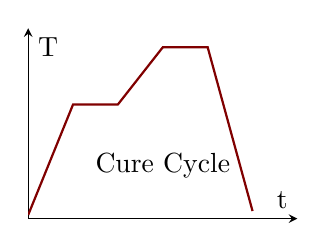
\begin{tikzpicture}
    \begin{axis}[
        width=5cm, height=4cm,
        xlabel={t}, ylabel={T},
        grid=both, 
        axis lines=middle, 
        xtick=\empty, ytick=\empty,
        ymin=0, ymax=5,
        xmin=0, xmax=6,
        legend style={at={(16.5,15.8)},anchor=north}
    ]
    % Line plot: positive ramp, horizontal, positive ramp, horizontal, negative ramp
    \addplot[thick, maroon] coordinates {
        (0,0.1) 
        (1,3)  % Positive ramp
        (2,3)       % Horizontal line
        (3,4.5)       % Positive ramp
        (4,4.5)       % Horizontal line
        (5,0.2)      % Negative ramp
    };
    \node at (axis cs: 3, 1.4) {Cure Cycle};
    \end{axis}
\end{tikzpicture}
};

% --- Nodes ---
% Inputs to the PINO Model
\node (ht) at(9.75,-2) [process2] {$h_{top}$};
\node (hb) at(11,-2) [process2] {$h_{bottom}$};
\node (Lt) at(12.25,-2) [process2] {$L_{t}$};
\node (plus) at(11,-1.4) {$+$};

% Curly bracket around the three nodes
\draw [decorate,decoration={brace,amplitude=8pt,mirror}] 
  (ht.south west) -- (Lt.south east) node [black,midway,xshift=0.4cm]{};
\node (designtitle) at(11,-3.3) {\textit{Tool and Equipment}};
\node (designtitle) at(11,-3.6) {\textit{Design Variable}};


%

% Add feedback line
\draw[->, thick] (6, -4) -- (6, -4.5) -- (-2, -4.5) -- (-2, -1.25);
\node (feedbacktext) at(2,-4.3) {\textit{Updated design}};
\node (loss1) at(4.2,-1) {\textit{Evaluate}};
\node (loss2) at(4.2,-1.5) {\textit{losses}};

% captions
\node (Initial Design) at(-5,1.7) {\textit{Initial Design}};
\node (PIDON) at(1,1.7) {\textit{PIDON Model}};
\node (Optimizer ) at(6,1.7) {\textit{Optimizer}};
\node (Optimum Design ) at(11,1.7) {\textit{Optimal Design}};

\end{tikzpicture}
\caption{An accelerated gradient-based design optimization framework: Using the PIDON model, the framework predicts the spatio-temporal evolution of part temperature and DOC, calculates the loss, and iteratively adjusts design variables through gradient-based optimization to find the optimal design.}
\label{fig:pino_framework}
\end{figure}
\subsubsection{Problem Formulation}
As elaborated in subsection \ref{composites}, we consider nine design variables (i.e., six parameters related to the cure cycle and three associated with tool/equipment design) represented as: $u = [r_1, r_2, hd_1, hd_2, ht_1, ht_2, h_{top}, h_{bot}, L_t]$. The optimization problem is formulated to minimize a total loss function \(\mathcal{L}(u)\), composed of four individual loss terms representing the objectives defined in the above subsection:
\begin{equation}
  \mathcal{L}(u) = \mathcal{L}_{1}(u) +  \mathcal{L}_{2}(u) + \mathcal{L}_{3}(u) +\mathcal{L}_{4}(u)  
\end{equation}
Using the PIDON model as a surrogate, we predict part temperature and DOC, used in the loss calculations. For the first objective, a penalty function is defined based on the desired DOC. A penalty function ensures the DOC remains within the desired range of 0.85 to 0.95. If the DOC falls outside this range: either the minimum of DOC across the laminate is below 0.85 or the maximum of DOC across the laminate exceeds 0.95, a penalty is applied; otherwise, the loss is zero.This can be expressed as:
\begin{equation}
\mathcal{L}_1(u) = 
\begin{cases} 
\left| 0.85 - \min(G^{\alpha}_{\theta}(u)(y_{t})) \right|, & \text{if } \min(G^{\alpha}_{\theta}(u)(y_{t})) < 0.85; \\
\left| \max(G^{\alpha}_{\theta}(u)(y_{t})) - 0.95 \right|, & \text{if } \max(G^{\alpha}_{\theta}(u)(y_{t})) > 0.95; \\
0, & \text{else}.
\end{cases}
\end{equation}
Here, \( y_t = [t|_{t=t}, z] \) and \( z \) is the collocation points in the spatial domain \( z \). A second objective is to minimize the gradient of the DOC across the laminate at the end of the curing process. Since the PIDON model is differentiable, the gradient is computed using automatic differentiation across the laminate thickness, and it is then averaged. This can be expressed as follows:
\begin{equation}
\mathcal{L}_2(u) = \frac{1}{N_z} \sum_{i=1}^{N_z} \left| \frac{\partial (G^{\alpha}_{\theta}(u)(y_{t}^{(i)}))}{\partial z}  \right|
\end{equation}
Here, \( N_z \) is the number of collocation points along the \( z \)-coordinate. The third objective ensures that the maximum part temperature does not exceed 185°C. Hence, a penalty function is introduced as follows:
\begin{equation}
\mathcal{L}_3(u) = \begin{cases} 
\left| 185 - \max(G^{T_{t}}_{\theta}(u)(y)) \right|, & \text{if } \max(G^{T_{t}}_{\theta}(u)(y)) > 185; \\
0, & \text{else.}
\end{cases}
\end{equation}
The fourth objective aims to limit the thermal lag to values below 20°C. This objective can be expressed as follows:
\begin{equation}
\mathcal{L}_4(\mathbf{\phi}) = \frac{1}{N} \sum_{i=1}^{N} \begin{cases} 
\left| 20 - (T_{a}(y^{(i)}) - G^{T_{t}}_{\theta}(\mathbf{\phi})(y^{(i)})) \right|, \\
\text{if } (T_{a}(y^{(i)}) - G^{T_{t}}_{\theta}(\mathbf{\phi})(y^{(i)})) > 20; \\
0, \text{else.}
\end{cases}
\end{equation}
\subsubsection{Optimizer}
The optimization problem for the inverse design of composites autoclave processing is formulated as:
as follows:
\begin{equation}
\begin{aligned}
    u^* &= \arg \min_{u} \mathcal{L}(u), \\
    \text{subject to:} \quad &u_{\text{min}} \leq u \leq u_{\text{max}}.
\end{aligned}
\label{eq:optimization_problem}
\end{equation}
The bounds \(u_{\text{min}}\) and \(u_{\text{max}}\) define the feasible design space for the design variables \(u\) and are summarized in Table \ref{tab:designRange}. They are typically defined by the inherent physical constraints of the process, such as the range of HTCs and temperature achievable by the autoclave oven. These constraints also align with the ranges of the input functions used during the training of the PIDON model. By adhering to these bounds, the design variables remain within the range of values on which the PIDON model was trained, ensuring it provides accurate and reliable predictions. The solution \(u^*\) represents the optimal set of design parameters that minimizes the total loss \(L(u)\),  while satisfying all objectives, constraints, and bounds. 

To solve this optimization problem, we employ a gradient-based approach, leveraging the differentiability of the PIDON model. Gradient-based methods are particularly advantageous for differentiable objective functions, as they use gradient information to efficiently explore the design space \citep{allen2022physical,um2020solver}. In this case, the loss function depends on the output of PIDON, which itself is a function of the input (i.e., design variables). By leveraging automatic differentiation, we can compute the gradient of the loss with respect to the design variables by propagating the gradients through the PIDON using the chain rule. These methods converge with fewer function evaluations, making them computationally efficient compared to sampling-based or heuristic approaches \citep{allen2022physical}. Specifically, we apply the Adam optimizer \citep{kingma2014adam}, which adapts the learning rate during optimization, improving the convergence speed and stability.

The optimization process involves the following steps (Figure \ref{fig:pino_framework}):
\begin{enumerate}
    \item \textbf{Initial Guess:} Select the initial design parameters $u^{0}$, either randomly or based on domain knowledge, and pass them to the PIDON model.
    \item \textbf{Forward Prediction:} Use the PIDON model to predict the spatio-temporal evolution of part temperature and DOC across the laminate based on the current design variables.
    \item \textbf{Loss Evaluation:} Compute the individual loss functions based on the predicted temperature and DOC values.
    \item \textbf{Gradient Computation:} Utilize automatic differentiation to compute the gradients of the total loss function \(\mathcal{L}(u)\) with respect to the design parameters \(u\). This step involves back-propagating the gradients through the PIDON model.
    \item \textbf{Update Design Variables:} Apply a gradient-based optimizer (e.g., Adam) to update the design variables \(u\) in the direction that minimizes the loss function using the computed gradients.
\end{enumerate}
Design variables are clipped within the specified bounds presented in Table \ref{tab:designRange} to prevent erroneous predictions. If a variable exceeds the upper limit, it is clipped to the upper value; if it falls below the lower bound, it is clipped to the lower limit. Each loss function is normalized to maintain consistent scales and prevent dominance of any objective. To compare efficiency, we implemented Nesterov-Adam (NAdam), PSO, and GA, using the same PIDON model and loss calculation procedure as the Adam optimizer for consistency.
\section{Results and Discussion}
\subsection{Validation of PIDON Model}
To train the PIDON model, the time domain was divided into 11 subdomains with various lengths, accommodating the level of complexity within each subdomain. All PIDON models used an identical architecture, as detailed in Table \ref{tab:hyperparameter}. We trained the model with 600 random input parameter combinations (i.e., input functions) spanning a wide range of values (Table \ref{tab:designRange}). We evaluated the model against finite element simulations as ground truth across five different test cases. Specifically, the part temperature and degree of cure (DOC) at the midpoint of the composite for a given set of input functions are compared with FE simulation results, as illustrated in Figure \ref{fig:pino_pred}. The plot demonstrates that the PIDON model provides highly accurate predictions, with its results closely overlapping those of the FE simulations. We also benchmarked its performance against previously developed operator-based models for composites processing, namely the Physics-Informed Neural Operator (PINO) \cite{ramezankhani2025advanced} and the physics-informed Fourier Neural Operator (FNO) \cite{meng2023novel} (Table \ref{tab:pidon_comparison}). We used mean absolute error (MAE) and mean maximum error as the evaluation metrics to compare model predictions with finite element simulations. The MAE was computed by averaging the absolute errors within and across all test cases. The mean maximum error was obtained by averaging the maximum errors from each test case. The results clearly show that the PIDON outperforms both PINO and FNO models, achieving MAE and mean maximum error that are approximately 50\% lower than those reported for the other models, despite being trained on a wider range of input functions. This demonstrates the superior accuracy and reliability of the proposed PIDON approach for predicting temperature and DOC in composite systems.

\begin{table}[]
\centering
\caption{Comparison of our proposed PIDON (ours), PINO \cite{ramezankhani2025advanced}, and FNO \cite{meng2023novel} based on mean absolute error(MAE) and maximum error (MAX) for temperature and DOC predictions.}
\begin{tabular}{@{}c|cc|cc|cc@{}}
\toprule
\multirow{2}{*}{Variable} & \multicolumn{2}{c|}{PIDON (ours)}     & \multicolumn{2}{c|}{PINO}      & \multicolumn{2}{c}{FNO}        \\ \cmidrule(l){2-7} 
                          & \multicolumn{1}{c|}{MAE} & MAX & \multicolumn{1}{c|}{MAE} & MAX & \multicolumn{1}{c|}{MAE} & MAX \\ \midrule
$T_{c}$(°C) & \multicolumn{1}{c|}{0.189} & 0.94  & \multicolumn{1}{c|}{0.362} & 2.231 & \multicolumn{1}{c|}{0.226} & 3.2  \\ \midrule
$\alpha$    & \multicolumn{1}{c|}{0.001} & 0.008 & \multicolumn{1}{c|}{0.002} & 0.02  & \multicolumn{1}{c|}{0.008} & 0.03 \\ \bottomrule
\end{tabular}
\label{tab:pidon_comparison}
\end{table}

\begin{figure}[]  
    \centering
    \includegraphics[width=0.48\textwidth]{01142025_pino_validation_plot.pdf} 
    \caption{Comparison of predicted part temperature and DOC from the PIDON model with FE simulation at the midpoint of the composite.}     % Caption for the figure
    \label{fig:pino_pred}                             % Label for referencing the figure
\end{figure}

\begin{table}[]
\centering
\caption{Performance comparison between gradient-based (i.e., Adam and NAdam)  and gradient-free  (i.e., PSO and GA) optimization models, highlighting computational time, PIDON Model calls and optimization objective metrics. Gradient-based optimizer results are averaged over 10 initial guesses, while gradient-free results use a single run. Model calls indicate the total number \texttt{(forward + backward)} function calls per optimization iteration.}
\begin{tabular}{@{}c|c|c|c|c|c|c@{}}
\toprule
Optimizer &
  \begin{tabular}[c]{@{}c@{}}Time \\ (Min.)\end{tabular} &
  \begin{tabular}[c]{@{}c@{}}Model Calls \\ (per iteration)\end{tabular} &
  \begin{tabular}[c]{@{}c@{}}Mean DOC \\ Gradient\end{tabular} &
  \begin{tabular}[c]{@{}c@{}}Max. $T_c$\\(=\textless{}185)\end{tabular} &
  \begin{tabular}[c]{@{}c@{}}Mean \\ Thermal Lag\\ (=\textless{}20)\end{tabular} &
  \begin{tabular}[c]{@{}c@{}} Mean DOC\\ (\textgreater{}=0.85)\end{tabular} \\ \midrule
\textit{Adam}  & 20.37 & \(1+2\)  & 0.0044±0.0002 & 185.21±0.25 & 14.10±0.67 &  0.853±0.0002      \\ \midrule
\textit{NAdam} & 20.02 & \(1+2\) &  0.0043±0.0001 & 185.12±0.16 & 14.16±0.61 &  0.852±0.00008       \\ \midrule
\textit{PSO}   & 58.7  & \(10 \times (1+1)\) & 0.0057        & 185.18      & 14.11      & 0.847  \\ \midrule
\textit{GA}    & 69.03 & \(100 \times (1+1)\) & 0.0045        & 185.07      & 14.91 & 0.852  \\ \bottomrule
\end{tabular}
\label{tab:optimizer_comparison}
\end{table}
\subsection{Design Optimization via Differentiable Neural Operator}
\begin{figure*}[t]  
    \centering
    \includegraphics[width=1\textwidth]{loss_cure_cycyle_combined_no_white_space.pdf} 
    \caption{a) Evolution of the total loss during each iteration of the optimization process using the Adam optimizer. b) Comparison of the initial and optimized cure cycle profiles using the Adam optimizer, including the part temperature ($T_c$) behavior at the midpoint. c) DOC evolution across the laminate thickness from the initial (blue) to optimized (red) design variables. All results correspond to the optimization process with an initial guess for the design parameters \(u^{0} = [2.5, 1.5, 56, 117, 112, 176, 75, 100, 2.2]\).}
    \label{fig:loss_cure_cyce}                             % Label for referencing the figure
\end{figure*}
\begin{figure*}[t]  
    \centering
    \includegraphics[width=1\textwidth]{01172025_paper_constarints_with_diff_inti_condition.pdf} 
    \caption{Evolution of key metrics during optimization: a) Average DOC across the laminate thickness, b) Maximum Temperature observed in the laminate, c) Average Axial Cure Gradient, and d) Average Thermal Lag, at each optimization step. Results are averaged over 10 different initial guesses, with shaded bands representing ± standard deviation to indicate variability across the optimization runs.}     % Caption for the figure
    \label{fig:constraints}                             % Label for referencing the figure
\end{figure*}
A trained PIDON model is used as a surrogate model to identify the optimal design parameters for the autoclave curing process. Losses are evaluated using a 20×100 grid of collocation points, with 20 points in the spatial domain ($z$) and 100 in the time domain. The performance of the framework was evaluated for two composite part thicknesses: 20 mm, as discussed in this section, and 30 mm, which is detailed in Appendix \ref{30mm}. Figure \ref{fig:loss_cure_cyce} shows the key outcomes of the optimization procedure for a random initial state \(u^{0} = [2.5, 1.5, 56, 117, 112, 176, 75, 100, 2.2]\). Figure \ref{fig:loss_cure_cyce}.a shows the evolution of the total loss during each iteration of the optimization process using the Adam optimizer. Figure \ref{fig:loss_cure_cyce}.b compares the initial and optimized cure cycle profiles, including the part temperature behavior at the midpoint of the composite. Although the air temperature is higher for the optimized design compared to the initial design, the maximum part temperature remains below the threshold in both cases. The initial and optimal DOC distributions across the laminate thickness are compared in Figure \ref{fig:loss_cure_cyce}.c. In the initial design, the DOC remains way below the 0.85 threshold, while the optimized design achieves a DOC exceeding 0.85 across the entire laminate thickness. These results clearly demonstrate the effectiveness of the proposed framework in achieving substantial improvements in cure cycle performance. The optimization framework yields the optimized design variables $u^{*} = [2.61, 1.2, 70, 125, 119, 183.9, 52.68, 91.61, 2.75]$ which satisfies all objectives, ensuring a high-quality manufactured part. The total computation time for a single optimization run is 20.37 minutes.

The obtained optimal design aligns very well with the theoretical expectations. Specifically, a higher value of \(r_1\) and a lower value of \(r_2\) ensures efficient heating during the first ramp phase while preventing excessive heat buildup (caused by resin polymerization) during the second phase. The optimal design has the highest \(ht_1\) to maximize heat during the first hold, ensuring a cure rate above 0.85 while avoiding excess heat in the second hold. For \(L_t\), the optimal design has a mid-range value. While a higher tool thickness can help mitigate excessive exothermic reactions, it may lead to a non-uniform DOC across the laminate, thus the chosen thickness can balance these effects.

% In addition, the total computation time for a single optimization run is 20.37 minutes, highlighting the framework's efficiency.

Further, to demonstrate the robustness of our framework, we present the optimization results using Adam for 10 different initial guesses. The average objective evolution across these runs is shown in Figure \ref{fig:constraints}. The figure illustrates the progression of key objectives during optimization, including the average DOC across the laminate (Figure \ref{fig:constraints}.a), maximum part temperature (Figure \ref{fig:constraints}.b), average axial cure gradient (Figure \ref{fig:constraints}.c), and average thermal lag (Figure \ref{fig:constraints}.d). The blue line represents the mean value across the 10 initial guesses, while the shaded band indicates the standard deviation. From the figure, it is evident that in some initial designs, the DOC is below 0.85. However, the optimal designs consistently achieve a DOC exceeding 0.85 across the laminate thickness. Additionally, the variation in DOC across the thickness is significantly reduced in the optimized designs compared to the initial designs. This improvement is further reflected in the steady decrease of the DOC gradient with each optimization step. Since DOC and maximum part temperature are correlated, initial designs with higher DOC exhibit higher part temperatures. In the optimization process, the maximum part temperature, which initially varies widely, stabilizes precisely at 185°C in the optimized designs. Lastly, the average thermal lag successfully remains below 20°C throughout the optimization procedure.
\subsection{Comparison to gradient-free methods}
In addition to our proposed optimization framework, we implemented and compared alternative optimization techniques, including NAdam, PSO, and GA, to evaluate their performance. The NAdam was executed for 180 iterations. The PSO was implemented with a swarm of 20 particles, running for 25 iterations, while the GA utilized a population size of 100 and was executed for 100 iterations. The performance of these optimizers, along with their computation times, is summarized in Table \ref{tab:optimizer_comparison}. For gradient-based optimizers, such as Adam and NAdam, the results are averaged over 10 different initial guesses to assess robustness. For population-based optimizers, since they are less sensitive to initial guesses, a single optimization run was executed and reported. In terms of the achieved optimal states, the gradient-based and gradient-free methods resulted in comparable performance. In terms of the number of function calls during the optimization process, gradient-based methods call the PIDON model once for forward prediction and twice for backward propagation (axial DOC gradient calculation and optimizer gradient update) per iteration (1 + 2). In contrast, gradient-free methods require one forward and one backward call for axial DOC gradient calculation for each individual in the population per iteration \((1+1) \times p\), where \(p\) is the population size. This makes gradient-based optimizers significantly more efficient with fewer function evaluations during the optimization process. Hence, the gradient-based optimizers demonstrated a significant computational advantage, converging approximately \textit{three times} faster than their gradient-free counterparts. This clearly indicates the advantage of utilizing a differentiable neural operator model in conjunction with a gradient-based optimization approach for accelerated and robust design optimization in advanced manufacturing and materials processing applications.
\section{Conclusions}
In this work, we present an end-to-end accelerated design optimization framework for advanced engineering design, specifically developed for the autoclave curing process in composite materials processing. At the core of the framework is an enhanced PIDON model, specifically designed to capture the nonlinear dynamics of the autoclave process with high accuracy. The improved PIDON integrates a nonlinear decoder and temporal domain decomposition techniques, delivering superior performance compared to existing neural operator-based models across wide range of diverse input functions and extended temporal domains. By leveraging the differentiability of the trained PIDON model, the framework utilizes the gradient-based Adam optimizer to efficiently identify optimal design parameters. When benchmarked against gradient-free methods such as PSO and GA, the Adam optimizer achieves comparable performance while operating approximately three times faster. This enables the accelerated and accurate identification of optimal design states for the autoclave curing process. Furthermore, the framework is highly adaptable and can be extended to address other advanced engineering design challenges, making it well-suited for digital twin applications.

\documentclass{article}


\usepackage{arxiv}

\usepackage[utf8]{inputenc} % allow utf-8 input
\usepackage[T1]{fontenc}    % use 8-bit T1 fonts
\usepackage{hyperref}       % hyperlinks
\usepackage{url}            % simple URL typesetting
\usepackage{booktabs}       % professional-quality tables
\usepackage{amsfonts}       % blackboard math symbols
\usepackage{nicefrac}       % compact symbols for 1/2, etc.
\usepackage{microtype}      % microtypography
\usepackage{lipsum}
\usepackage{authblk}
\usepackage{graphicx}
\usepackage{amsmath}
\usepackage{comment}
\usepackage{xcolor}
\usepackage{adjustbox}
\usepackage{booktabs}
\usepackage{subcaption}
\usepackage{float}
\usepackage{algorithmic}
\usepackage{caption}

\title{Neural Network-based Vehicular Channel Estimation Performance: Effect of Noise in the Training Set}

\author[1,2,3]{\textbf{S.~A.~Ngorima}}
\author[1]{\textbf{A.~S.~J.~Helberg}}
\author[1,2,3]{\textbf{M.~H.~Davel}}

\affil[1]{Faculty of Engineering, North-West University, South Africa}
\affil[2]{Centre for Artificial Intelligence Research, South Africa}
\affil[3]{National Institute for Theoretical and Computational Sciences, South Africa}

\renewcommand\Authands{ and } % Replace "and" with "and" for the last author

%\date{}
%\date{\vspace{-2em}}

\begin{document}

\maketitle

\begingroup
\renewcommand{\thefootnote}{}
\footnote{This work is a preprint of a published paper by the same name\cite{10.1007/978-3-031-78255-8_12}. The authenticated version is available online at \url{https://doi.org/10.1007/978-3-031-78255-8_12}.}
\endgroup

\begin{abstract}
Vehicular communication systems face significant challenges due to high mobility and rapidly changing environments, which affect the channel over which the signals travel. To address these challenges, neural network (NN)-based channel estimation methods have been suggested. These methods are primarily trained on high signal-to-noise ratio (SNR) with the assumption that training a NN in less noisy conditions can result in good generalisation. This study examines the effectiveness of training NN-based channel estimators on mixed SNR datasets compared to training solely on high SNR datasets, as seen in several related works. Estimators evaluated in this work include an architecture that uses convolutional layers and self-attention mechanisms; a method that employs temporal convolutional networks and data pilot-aided estimation; two methods that combine classical methods with multilayer perceptrons; and the current state-of-the-art model that combines Long-Short-Term Memory networks with data pilot-aided and temporal averaging methods as post processing. %Our results indicate that a training dataset with a high SNR is not always optimal, and the training SNR levels should be considered a hyperparameter to be adjusted. 
Our results indicate that using only high SNR data for training is not always optimal, and the SNR range in the training dataset should be treated as a hyperparameter that can be adjusted for better performance. This is illustrated by the better performance of some models in low SNR conditions when trained on the mixed SNR dataset, as opposed to when trained exclusively on high SNR data.
\end{abstract}


% keywords can be removed
\keywords{Channel estimation \and deep learning \and neural networks \and CNN-Transformer \and IEEE 802.11p \and vehicular channels.}

\section{Introduction}
The integration of network infrastructure with artificial intelligence (AI) is becoming more prevalent due to the increasing demands of data-intensive applications and the need for more efficient and reliable communication systems. Incorporating AI into these systems promises to improve network management, resource allocation, and overall system performance.

This convergence is notably evident in vehicular communication, which is an important component of intelligent transportation systems. Vehicular communication systems face unique problems due to their high mobility, rapidly varying environments, and significant latency requirements. One of the challenges in this domain is obtaining accurate channel estimates, which is critical to ensuring reliable communication between vehicles and infrastructure. Channel estimation involves determining the characteristics of a communication channel and monitoring its changes to adjust to varying conditions~\cite{875230}.
%This is particularly evident in vehicular communication, where one of the most significant challenges is accurate channel estimation. 

The dynamic nature of vehicular environments, characterised by rapidly changing channel conditions, poses a challenge to traditional channel estimation methods. These methods include methods such as least squares (LS) and minimum mean square error (MMSE), which rely on mathematically estimating the channel based on the received version of known data sent as a preamble to the signal. Although effective in more stationary environments, these techniques often struggle to keep up with the rapid changes inherent in vehicular channels~\cite{gizzini2020deep}. This limitation highlights the need for more advanced adaptive approaches to channel estimation in these high-mobility scenarios. 

In recent years, researchers have increasingly focused on using data symbols directly to estimate the channel in a method referred to as data pilot-aided (DPA) channel estimation. DPA estimation addresses the challenges posed by dynamic environments, especially in vehicular communication systems, where pilot signals are evidently insufficient. Unlike traditional methods that rely heavily on a fixed number of pilot signals for channel estimation, DPA estimation uses demapped data symbols as additional pilots. This approach allows for more flexible and adaptive tracking of channel variations without the need to allocate more resources for pilot signals, thereby improving efficiency and accuracy in rapidly changing channels. However, the performance of the DPA method can be significantly affected by errors introduced during the demapping process, which may limit its overall effectiveness~\cite{pan2021channel}.
%However, the DPA method has a demapping error that significantly limits its performance~\cite{pan2021channel}. 
To improve efficiency, DPA estimation is typically used with an error compensation scheme to reduce channel distortion and prevent errors from propagating to the next symbols in a frame. Two common error compensation approaches for channel estimation are spectral temporal averaging (STA)~\cite{fernandez2011performance} which utilises the correlations of data symbols in time and frequency domains to estimate the channel and time-domain reliable test frequency domain interpolation (TRFI)~\cite{kim2014time}, as described in more detail in Section \ref{well-known}. 
However, these methods still struggle in highly dynamic scenarios~\cite{gizzini2021temporal}.

Deep learning (DL) has recently gained attention for its ability to improve the accuracy of channel estimates. A method utilising autoencoders and training on a high signal-to-noise ratio (SNR) dataset (SNR=40 dB) was proposed to correct DPA estimate errors in the frequency domain~\cite{han2019deep}. However, it did not account for temporal changes, limiting its performance. Furthermore, incorporating feedforward networks into classical methods such as STA and TRFI methods, as proposed in~\cite{gizzini2020deep}, has shown promise in improving estimation accuracy. These methods were also trained on high SNR datasets (SNR=30 dB).
 
These methods offer valuable baselines.
%Nevertheless, these methods are not effective on all signal-to-noise ratio SNRs. 
Recently, a long-short-term memory (LSTM)-based architecture has been proposed to capture the temporal and frequency characteristics of vehicular channels~\cite{gizzini2021temporal}. This method was trained on a dataset generated at the SNR level of 40 dB and demonstrated significant improvements over previous estimators. However, this method is computationally expensive. 

This study introduces the use of a mixed SNR dataset, where the training dataset includes data generated at different SNR levels. We hypothesise that training on a mixed SNR dataset helps an neural network (NN) generalise across a wider range of real-world conditions by exposing it to both noise-dominated and signal-dominated scenarios. This approach contrasts with the methodology adopted in several studies~\cite{gizzini2020deep,gizzini2020joint,gizzini2021temporal,pan2021channel}, which propose that training the NN-based estimator using a dataset generated only at a high SNR level enhances its ability to generalise in any environment: at high SNR the impact of the channel is greater than the impact of noise, therefore it is expected that the NN develops better channel knowledge. 

We evaluate the use of the mixed SNR dataset using a CNN-Transformer-based  estimator~\cite{Ngorima2024a} which is a hybrid model that combines a one-dimensional convolutional neural network (CNN) with a transformer architecture, a TCN-DPA estimator~\cite{Ngorima2024} that uses a temporal convolutional network (TCN) to correct the DPA propagation error, two estimators based on concatenating a multilayer perceptron (MLP) with a classical method, in this case STA-MLP~\cite{gizzini2020deep} and TRFI-MLP~\cite{gizzini2020joint}, and the LSTM-DPA-TA method~\cite{gizzini2021temporal} which combines Long Short-Term Memory (LSTM) networks with Data Pilot-Aided (DPA) estimation and Temporal Averaging (TA).


\section{Background}

We describe the system model, well-known channel estimation schemes in vehicular communications, and some of the NN-based channel estimation techniques currently used. 
We also provide a brief description of the IEEE 802.11p physical layer structure that is used in all simulations, along with a description of its specifications. 

\subsection{System Model}
\label{system_model}

In this paper, we adopt the IEEE 802.11p physical layer structure, which is specifically designed for vehicular communication systems. This section follows a detailed discussion of the IEEE 802.11p specifications as outlined in Ngorima et al.~\cite{Ngorima2024}. %We also provide a detailed discussion of some of the channel estimation methods later used for this work's evaluation stage.
%
The IEEE 802.11p standard uses Orthogonal Frequency Division Multiplexing (OFDM) to transfer data by dividing the available bandwidth into several subcarrier frequencies for simultaneous transmission of multiple signals. 52 of the 64 available subcarriers are used for data transmission and pilot symbols. The remaining subcarriers are for guard bands and direct current (DC) offset. To illustrate this structure, Figure \ref{fig:1DCNN} shows the IEEE 802.11p OFDM frame, indicating pilot and data subcarriers.

\begin{figure}[ht]
    \centering
    \includegraphics[width=0.5\linewidth]{images/1DCNN.jpg}
    \caption{The IEEE 802.11p frame structure, illustrating the allocation of subcarriers for pilot and data transmission.}
    \label{fig:1DCNN}
\end{figure}
In this work, we consider a frame structure that consists of two preamble symbols for signal detection and timing synchronisation, followed by a signal field that contains transmission parameters.
The received signal on subcarrier $[k]$ at time $i$ can be represented as
%
\begin{equation*} Y_{i}[k]=H_{i}[k]X_{i}[k]+N_{i}[k],\tag{1} \label{rec_signal}\end{equation*}
%
where $H_i[k]$, $X_i[k]$ and $N_{i}[k]$ denote the respective channel response, transmitted signal, and additive Gaussian noise (AWGN), respectively. Note that in vehicular channels $H_{i}$ varies in both the time and frequency domains.

\subsection{Well-known Vehicular Channel Estimation Schemes}
\label{well-known}
This section describes some of the main vehicular channel estimation schemes that have been widely used and studied in the literature. These methods were selected based on their effectiveness in dynamic environments and their foundational role in the development of more advanced NN-based estimators.
%The following are some of the vehicular channel estimation schemes. 

\subsubsection{DPA Estimation:}
The first step of the DPA process, as described by Pan et al.~\cite{pan2021channel}, is to calculate the initial estimate of the frame. This is done by applying the least squares (LS) estimation to the preamble as shown below:

% \subsubsection{DPA Estimation}

% The first step of the DPA process is to calculate the initial estimate of the frame. This is done by applying the least squares (LS) estimation to the preamble as shown below:

\begin{equation*} \hat { {h} }_{\text {0}}[k] = \frac { {y} ^{(p)}_{1}[k] + {y} ^{(p)}_{2}[k]}{2 {p} [k]}, \tag{2}\label{eqn:ls}\end{equation*}
%
where ${y} ^{(p)}_{1}[k]$ and ${y} ^{(p)}_{2}[k]$ are the known orthogonal preambles received on the $[k]$ subcarrier and $p[k]$ is the OFDM data symbol transmitted over the k-th subcarrier.
%
The next OFDM symbols in the frame are equalised using the initial estimate as the starting point as follows:
%
\begin{equation*} y_{i}^{\text{eq}}[k]= \frac{y_{i}[k]}{\hat{h}_{i-1}^{\text{DPA}}[k]},\hat{h}_{0}^{\text{DPA}}[k]=\hat{h}_{\text {0}}[k].\tag{3}\label{eqn:yeq}\end{equation*}
%
The equalised symbol is demapped and mapped to its closest constellation point as: %(see (\ref{eqn:conse})). 
%
\begin{equation*}d_{i}[k]=\mathfrak{R}\left(\frac{y_{i}[k]}{ \hat{h}_{i-1}^{\text{DPA}}[k]}\right), \hat{h}_{0}^{\text{DPA}}[k]=\hat{h}_{\text {LS}}[k],\tag{4}\label{eqn:conse}\end{equation*}
%
Finally, the DPA channel is updated: 
%
\begin{equation*}\tilde{h}_{\mathrm{D}\mathrm{P}\mathrm{A}_{i}}[k]=\frac{y_{i}[k]}{d_{i}[k]}\tag{5}\end{equation*}
%
\subsubsection{STA Estimation Scheme:}
%
STA uses both spectral (frequency) and temporal correlations within data symbols to estimate the channel~\cite{gizzini2020deep}. STA can also be viewed as a recursive filtering process that combines multiple channel estimates into a more accurate estimate.
%
The first step is to calculate a channel estimate in the frequency domain $\hat{h}{i}^{\text{FD}}[k]$ as follows: 
%
\begin{equation*} \hat{h}{i}^{\text{FD}}[k]=\sum{\lambda=-\beta}^{\beta}\omega_{\lambda}\hat{h}_{i}^{\text{DPA}}[k+\lambda],~\omega _{\lambda } = \frac {1}{2\beta +1},\tag{6}\end{equation*}
%
where $2\beta + 1$ represents the number of subcarriers that are considered.
%
Subsequently, a temporal average is computed to arrive at the final STA channel estimate, $\hat{h}{i}^{\text{STA}}[k]$:
%
\begin{equation*}\hat{h}{i}^{\text{STA}}[k]=\left(1-\frac{1}{\alpha}\right)\hat{h}{i-1}^{\text{STA}}[k]+\frac{1}{\alpha}\hat{h}_{i}^{\text{FD}}[k],\tag{7}\end{equation*}
%
where $\alpha$ is a smoothing parameter that controls the weight given to current and previous estimates.

\subsubsection{TRFI Estimation Scheme:}
%
TRFI leverages the high correlation within OFDM symbols to improve the accuracy of the channel estimation~\cite{gizzini2020joint}. The process starts by creating multiple channel estimates for each symbol using the DPA method. The received symbol is equalised using the estimates of the current and previous symbols ($\hat{h}_{i}^{\text{DPA}}[k]$) and ($\hat{h}_{i-1}^{\text{DPA}}[k]$) respectively.
%
\begin{align*}
{y}_{i-1}^{\text{eq}\prime}[k] &= \frac{y_{i-1}[k]}{\hat{h}_{i}^{\text{DPA}}[k]}, \\
{y}_{i-1}^{\text{eq}\prime\prime}[k] &= \frac{y_{i-1}[k]}{\hat{h}_{i-1}^{\text{DPA}}[k]}, \tag{8}\label{eqn:cdp_eq}
\end{align*}
%
Subsequently, the equalised symbols are remapped to their corresponding constellation points, ${d}_{i-1}^\prime[k]$ and ${d}_{i-1}^{\prime\prime}[k]$. 
%
TRFI then categorises subcarriers into reliable and unreliable sets based on a reliability test between the remapped symbols. Subcarriers with consistent remapped symbols, that is, ${d}_{i-1}^\prime[k]= {d}_{i-1}^{\prime\prime}[k]$, are considered reliable, while those with discrepancies are classified as unreliable. TRFI then interpolates channel estimates for unreliable subcarriers by using the reliable subcarriers as anchor points. This interpolation process effectively fills in the gaps in channel knowledge, resulting in a more accurate overall channel estimate. A detailed discussion on the interpolation procedure is given in~\cite{gizzini2020deep}.
%
\subsection{MLP-based Estimators} 
To enhance the performance of conventional STA and TRFI estimators, Gizzini et al.~\cite{gizzini2020deep} introduced MLP-based channel estimation methods. In these methods, MLP layers are added to the STA and TRFI processes, allowing the model to learn complex patterns in vehicular channels and thereby improve the accuracy of the estimation. The methods STA-MLP and TRFI-MLP initially conduct DPA estimation, proceed with STA or TRFI estimation and subsequently feed the results into the MLP layers. 
%
\subsection{TCN-DPA Estimator}
%
As proposed in~\cite{Ngorima2024}, the TCN-DPA estimator integrates a Temporal Convolutional Network (TCN) with DPA estimation to enhance channel estimation in dynamic environments. The TCN processes the received OFDM symbols in the frequency domain, treating subcarriers as time steps. The extracted features are then passed to the DPA process, where the previous TCN output, \(\hat{h}_{i-1}^{\text{TCN}}[k]\), is used to equalise the current received symbol. After equalisation, the symbol is demapped and remapped to the nearest constellation point to obtain the final channel estimate, \(\hat{h}_{i}^{\text{TCN}}[k]\). This estimate is updated iteratively using the DPA process. This approach leverages the ability of the TCN to model long-range dependencies across subcarriers, making it effective for complex channel conditions.

\subsection{LSTM-DPA-TA Estimator}
%
The LSTM-DPA-TA estimator~\cite{gizzini2021temporal} integrates an LSTM network with DPA and Temporal Averaging (TA) techniques to enhance channel estimation in vehicular environments. In this approach, the LSTM processes the received OFDM symbols to extract key features, which are then passed into the DPA module. The resulting channel estimates are further refined using the TA technique. In the LSTM-DPA-TA method, OFDM symbols are treated as time steps, with subcarriers considered as features within each time-step sequence. This design enables the model to effectively capture frequency dependencies and improve the accuracy of channel estimation under dynamic conditions.

\subsection{CNN-Transformer}
The CNN-Transformer is a recently proposed hybrid architecture for vehicular channel estimation in~\cite{Ngorima2024a}. This approach combines the strengths of CNNs and Transformer networks to analyse vehicular channel data comprehensively. The channel data can be represented in both the time and frequency domains. The frequency domain represents the subcarriers of the OFDM symbols, while the time domain represents the sequence of OFDM symbols transmitted over time. Each OFDM symbol is transmitted across multiple subcarriers. %, which are essentially distinct frequency bands. 
The frequency domain captures the spatial characteristics of the channel across OFDM subcarriers, while the time domain reflects the temporal dynamics as OFDM symbols are transmitted sequentially. 

In this CNN-Transformer architecture, subcarriers are treated as the `time steps'. 
The architecture leverages CNNs to extract local features from subcarriers and uses Transformer layers to capture global dependencies across the frequency domain. The CNN component applies 1D convolutions to capture local patterns, while the Transformer component uses self-attention mechanisms to analyse patterns between subcarriers globally.

\section{Methodology}
\label{proposed}

This section outlines the methodological framework used in this study.
%to assess the best training practices for different NN-based channel estimators. 
We start with a detailed description of the datasets used for training and evaluation, specifically focussing on two approaches: the mixed SNR dataset and the high SNR dataset. Following this, we discuss the data preprocessing steps applied to transform complex received symbols into a format suitable for input into NNs. 
%
%
\subsection{Data Preparation}
\label{dataprep}
We simulate vehicle-to-vehicle communication following the `Vehicle-To-Vehicle Expressway Same Direction with Wall' (VTV-SDWW) channel model~\cite{4526014}. Our simulation specifically modelled vehicles moving at 100 km/h, with a Doppler shift of 550 Hz. We used 16QAM (16-Quadrature Amplitude Modulation) modulation for data transmission in this urban environment scenario. This modulation scheme encodes the data by varying the amplitude and phase of the carrier signal.

\subsubsection{Mixed SNR Dataset}
The mixed SNR dataset represents a wide range of noise introduced on the VTV-SDWW channel. For this dataset, we simulate 18,000 time-specific frames with SNR values ranging from 0 to 40 dB in increments of 5 dB. Each SNR level includes 2,000 frames, with 50 OFDM symbols spread across 52 active subcarriers (48 data and 4 pilot subcarriers). During training, each model is exposed to the entire range of SNR levels.
%
The validation set is created by reserving 25\% of this training data to monitor the performance of the model during training. An independent test set consisting of 2,000 frames is generated separately from the training sets. This test set includes frames at SNR levels of 0, 5, 10, 15, 20, 25, 30, 35, and 40 dB, ensuring that the evaluation correctly reflects the performance across different SNR conditions. The same test set is used to test all the models regardless of how they are trained. 
%
\subsubsection{High SNR Dataset}
The high SNR dataset focusses on a fixed SNR level, representing less noisy or nearly ideal channel conditions, as opposed to the mixed SNR dataset. This dataset is used to train models with the assumption that training NNs in an environment with a clearly defined channel can lead to better generalisation even in noisy environments~\cite{gizzini2021temporal,gizzini2020deep,gizzini2020joint,pan2021channel}. 
In this work, the high SNR dataset consists of 18,000 time-specific frames, all generated at a 40 dB SNR level, with the same frame structure as the mixed SNR data. As before, 25\% of the training data is set aside for validation. 

\subsubsection{Data preprocessing}

To preprocess the data for NN models, we transform the complex 16QAM symbols received across subcarriers and time slots into a real-valued format. Each received symbol consists of both real and imaginary components. The following steps are performed to prepare the data:

\begin{enumerate}
    \item \textbf{Separate Real and Imaginary Components:} Decompose each complex 16QAM symbol into its real and imaginary parts. Handle the data as two separate real-valued matrices instead of a single complex-valued matrix. For a given OFDM symbol, where \(y[k] = r[k] + j \cdot i[k] \) represents the received complex value at subcarrier \( k \), extract \( r[k] \) as the real part and \( i[k] \) as the imaginary part.

    \item \textbf{Interleave Components:} After separation, interleave the real and imaginary components. This means arranging the real and imaginary parts in an alternating sequence across the time slots. By interleaving, a unified structure that preserves the relationship between the real and imaginary parts within the input data is created.

    \item \textbf{Form the Input Matrix:} Structure the interleaved data into a matrix with dimensions \( 52 \times 100 \), where 52 represents the number of subcarriers and 100 represents the sequence of interleaved real and imaginary components across the time slots. This transformation enables the NN to process the complex-valued input as a series of real-valued inputs.

    \item \textbf{Prepare Input Data for NN models:} The resulting matrix is now a real-valued representation of the original complex data, ready for input into NN models. %This preprocessing step ensures that the network can effectively learn from the data without being hindered by the challenges of handling complex numbers directly.
\end{enumerate}
%
The transformed input matrix described above is visually represented in Figure~\ref{fig:frame}. Each block in the figure represents the interleaved real and imaginary components of the received 16QAM symbols for a particular subcarrier across the OFDM symbols. 
The kernel size of 3 shown in the figure indicates the width of the sliding window used by the CNN during the convolution process across the subcarriers.
\begin{figure}[ht] 
    \centering
    \includegraphics[width=\linewidth]{images/Frame.jpg}
    \caption{Transformed IEEE 802.11p frame structure used as input to deep learning models, composed of 100 interleaved complex symbols and 52 subcarriers.}
    \label{fig:frame}
\end{figure}

\subsection{Hyperparameter Optimisation}
\label{sec:hyperparameters}
We reimplement most of the NN-based estimators discussed in the previous sections to ensure compatibility with our experimental setup and to be able to optimise each individually for the specific datasets used. Specifically, the CNN-Transformer, TCN-DPA, STA-MLP, and TRFI-MLP models were reimplemented from scratch. The LSTM-DPA-TA model is implemented using existing code available online. To verify the accuracy of our reimplementations, we compare the performance of our implementations against the benchmark results reported in the original studies, ensuring that they perform as expected.

The final architecture of each model is determined through a hyperparameter tuning process, to identify the optimal configurations for each model. We optimise the hyperparameters of all models in both datasets using Optuna, a Bayesian optimisation framework that efficiently searches the hyperparameter space using a tree-structured Parzen estimator (TPE)~\cite{akiba2019optuna}. This method systematically explores different hyperparameter configurations while conserving computational resources by early termination of underperforming trials. %The optimisation process covers a set of hyperparameters that address the important components of the model. %The steps in the optimisation procedure are as follows:

For each model, we conduct multiple trials with different random seeds to ensure that results are not biased by a particular initialisation. Specifically, we conduct 50 trials per model, each with 3 seeds, allowing us to assess the robustness of the selected hyperparameters. The search space for each model was designed to cover a wide range of potential configurations. The key hyperparameters include the learning rate, the number of layers, the layer size (kernel size,  number of attention heads, or layer width, depending on model), the learning rate scheduler parameters, and hyperparameters controlling regularisation through dropout. 
%The search space was determined on the basis of prior studies, domain knowledge, and preliminary experiments, ensuring that it was sufficiently broad to capture the optimal settings. 
During the optimisation process, we monitor the convergence of validation loss. Early stopping is employed to prevent overfitting, stopping training when the validation loss ceases to improve for a predefined number of epochs. 


\begin{table}[hb!]
\caption{Optimised hyperparameters for CNN-Transformer, TCN-DPA, STA-MLP, TRFI-MLP, and LSTM-DPA-TA on the mixed SNR and high SNR datasets.}
\label{tab:all_hyperparameters}
\centering
\begin{tabular}{lccc}
\hline
\textbf{Hyperparameter} & \hspace{0.15em}\textbf{Search Space} & \hspace{0.15em}\textbf{Mixed SNR}\hspace{0.15em} & \hspace{0.25em}\textbf{40 dB}\hspace{1em} \\
\hline
\multicolumn{4}{l}{\textbf{CNN-Transformer}} \\
Learning rate & [1e-5 to 1e-2] & 0.001 & 0.001 \\
Transformer layers & [1 to 4] & 2 & 4 \\
Number of attention heads & [1 to 4] & 2 & 4 \\
Hidden dimension & [64 to 128] & 128 & 128 \\
Dropout rate & [0.001 to 0.3] & 0.1 & 0.25 \\
Number of epochs & [50 to 200] & 110 & 200 \\
Number of CNN layers & [1 to 5] & 2 & 4 \\
CNN kernel size & [2 to 5] & 3 & 3 \\
\hline
\multicolumn{4}{l}{\textbf{TCN-DPA}} \\
Learning rate & [1e-5 to 1e-2] & 0.0006 & 0.003 \\
Number of Layers & [1 to 5] & 4 & 4 \\
Kernel Size & [2 to 5] & 2 & 2 \\
Dropout & [$10^{-5}$ to 0.5] & 0.17 & 0.01 \\
StepLR Step Size & [10 to 50] & 21 & 17 \\
StepLR Gamma & [0.5 to 1] & 0.9 & 0.8 \\
Epochs & [0 to 200] & 156 & 100 \\
\hline
\multicolumn{4}{l}{\textbf{STA-MLP}} \\
Learning rate & [1e-5 to 1e-2] & 0.001 & 0.001 \\
Number of layers & [1 to 5] & 2 & 3 \\
Size of hidden layer 0 & [5 to 30] & 29 & 15 \\
Size of hidden layer 1 & [5 to 30] & 27 & 15 \\
Size of hidden layer 2 & [5 to 30] & N/A & 15 \\
Total training epochs & [50 to 500] & 133 & 300 \\
\hline
\multicolumn{4}{l}{\textbf{TRFI-MLP}} \\
Learning rate & [1e-5 to 1e-2] & 0.0004 & 0.001 \\
Number of layers & [1 to 5] & 3 & 3 \\
Size of hidden layer 0 & [5 to 30] & 23 & 15 \\
Size of hidden layer 1 & [5 to 30] & 29 & 15 \\
Size of hidden layer 2 & [5 to 30] & 21 & 15 \\
Total training epochs & [50 to 500] & 130 & 160 \\
\hline
\multicolumn{4}{l}{\textbf{LSTM-DPA-TA}} \\
Learning rate & [1e-5 to 1e-1] & 0.004 & 0.01 \\
LSTM size & [64 to 128] & 128 & 128 \\
StepLR step size & [1 to 50] & 35 & 10 \\
StepLR step gamma & [0.1 to 1] & 0.7 & 0.8 \\
Training epochs & [50 to 500] & 160 & 500 \\
\hline
\end{tabular}
\end{table}

Table~\ref{tab:all_hyperparameters} provides a summary of the best hyperparameters obtained for each model across the datasets. In addition to the parameters in the table, batch normalisation is applied to enhance model generalisation. The Adam optimiser and a batch size of 128 was used for TCN-DPA, LSTM-DPA-TA, STA-MLP and TRFI-MLP. For the CNN-Transformer model, we use the AdamW optimiser and manually set the batch size to 16. 


\section{Results}
 This section evaluates the performance of channel estimators using BER as the primary metric. We compare the effectiveness of two training approaches: one using a mixed SNR dataset and the other using a high SNR dataset.  The evaluated architectures are CNN-Transformer, TCN-DPA, STA-MLP, TRFI-MLP, and LSTM-DPA-TA.

\subsection{BER}
BER is a crucial performance measure in digital communication. It compares transmitted and received bit sequences to assess system reliability. In channel estimation, a lower BER means more accurate signal reconstruction and fewer errors in decoded data. The following analysis details the BER performance of each model at different levels of SNR, providing a direct comparison between the two training approaches.
%\subsection{BER}
\begin{figure}[ht!]
    \centering
    \begin{subfigure}[b]{0.75\linewidth}
        \centering
        \includegraphics[width=\linewidth]{images/last_ber_bad.png}
        \caption{High SNR training dataset}
        \label{fig:high_snr_ber}
    \end{subfigure}
    \hfill
    \begin{subfigure}[b]{0.75\linewidth}
        \centering
        \includegraphics[width=\linewidth]{images/last_BER.png}
        \caption{Mixed SNR training dataset}
        \label{fig:mixed_ber}
    \end{subfigure}
    \caption{Comparison of BER performance for various channel estimators trained on high SNR and mixed SNR datasets. \label{fig:ber}}
\end{figure}

%Figures \ref{fig:high_snr_ber}. and \ref{fig:mixed_ber}. 
Figure~\ref{fig:ber} presents the BER performance of the channel estimators trained using a high SNR dataset (40 dB) and a mixed SNR dataset, respectively. The ideal curve, represented by the dotted black line in these figures, represents the best possible performance in channel estimation, where the received signal is assumed to be perfectly equalised without any channel estimation errors. This curve serves as a theoretical lower bound for the BER, showing the performance in a scenario where only additive white Gaussian noise (AWGN) is present and the channel effects are perfectly compensated for. The closer the BER of a model is to the ideal curve, the better its performance in accurately estimating the channel and mitigating the effects of noise. LS serves as the lower performance baseline. 

In Figure \ref{fig:high_snr_ber}, we observe several key trends across models trained on an high SNR dataset: 
In the low SNR range (0-10 dB), the STA-MLP and the LSTM-DPA-TA models perform relatively well, maintaining a lower BER compared to other models. %The LSTM-DPA-TA model also exhibits strong performance, achieving the lowest BER across this range, demonstrating its suitability for low SNR conditions when trained on high SNR data.
%
As we move into the mid SNR range (15-25 dB), the CNN-Transformer and DPA-TCN models show an improvement, particularly from 15 dB onwards, with performance becoming more pronounced from 20 dB. %The improvement becomes more exponential from 20 dB. 
This improvement at high SNR highlights that these models have effectively adapted to high SNR conditions. %arnt to less noisy conditions but not high noisy conditions. 
%TRFI-MLP also exhibits a steady increase in BER with increasing SNR, although its performance lags behind that of CNN-Transformer and DPA-TCN. This also indicates the limitation of training NNs with the high SNR dataset as the TRFI-MLP struggles to adapt to noisy conditions.
The TRFI-MLP model also improves in this range, although it lags behind the CNN-Transformer and DPA-TCN models, indicating some limitations in its ability to adapt to low SNR conditions.
% 
In the high SNR range (30-40 dB), the CNN-Transformer and DPA-TCN models continue to show further significant reductions in BER. The LSTM-DPA-TA model continues to outperform other models across all SNR levels, showing its effectiveness in less noisy conditions. In contrast, STA-MLP shows limited improvement beyond 20 dB, indicating that it struggles to capitalise on the reduced noise at higher SNR levels.

In the mixed SNR training scenario depicted in Figure \ref{fig:mixed_ber}, we observe that CNN-Transformer and DPA-TCN models exhibit excellent performance across the entire SNR range with CNN-Transformer outperforming all models.  %This suggests that these models are well-suited for a wide range of channel conditions when trained on mixed SNR datasets.
%
The LSTM-DPA-TA and STA-MLP models perform well at lower SNR levels (0 to 15 dB) but show reduced performance as the SNR increases, indicating diminished capabilities in high SNR conditions when trained on mixed SNR data. We can also observe the improved performance of the TRFI-MLP estimator across the entire SNR range tested compared to its performance when trained on the high SNR dataset. The unsatisfactory performance by LSTM-DPA-TA and STA-MLP indicates that while these models can handle varying noise conditions, they may not leverage mixed SNR training as effectively as TRFI-MLP, CNN-Transformer and DPA-TCN.

Models trained on mixed SNR data exhibit lower BER even in low-SNR scenarios, compared to those trained on high SNR data. Mixed SNR training appears to be beneficial for models such as TRFI-MLP, TCN-DPA, and CNN-Transformer, which show a significant improvement in low SNR conditions than when trained on high SNR. In contrast, the LSTM-DPA-TA and STA-MLP models demonstrate better performance when trained on a high SNR dataset, suggesting that these models make use of the better channel statistics available at high SNR. This is analysed in more detail below.

\subsection{Difference in BER Between Models Trained on Mixed SNR and High SNR Datasets}
Figure~\ref{fig:delta_ber} illustrates the difference in BER between models trained on high SNR datasets and those trained on a mixed SNR dataset. The graph clearly shows how the training dataset influences the performance of various models across different SNR ranges. In the low SNR range (0-10 dB), the CNN-Transformer and TCN-DPA models exhibit the highest positive delta, peaking around 10 dB. This indicates a substantial improvement in performance when these models are trained on a mixed SNR dataset compared to a high SNR dataset. A positive delta suggests that mixed SNR training better equips these models to generalise in low SNR conditions. TRFI-MLP also shows a noticeable positive delta, although less pronounced, indicating that mixed SNR training offers some advantages in low SNR environments. In contrast, the LSTM-DPA-TA and STA-MLP models display a slightly negative delta across this range, implying that training on high SNR datasets offers a marginal performance advantage in these specific models. 

As the SNR increases (15-25 dB), the positive delta values for the CNN-Transformer and TCN-DPA models start to decrease but remain positive, particularly around 15 dB. This indicates that while the benefits of mixed SNR training diminish slightly, these models still gain performance advantages in this SNR range. TRFI-MLP continues to maintain positive delta values, demonstrating that mixed SNR training consistently improves its performance at varying SNR levels. Meanwhile, the LSTM-DPA-TA model continues to show a negative delta, particularly at the higher end of the mid-SNR range, around 20-25 dB. Similarly, the STA-MLP model exhibits a slight negative delta in this range.

In the high SNR range (30-40 dB), the delta values for most models, including the CNN-Transformer, TCN-DPA, and TRFI-MLP, approach zero. This suggests that as the SNR increases and the impact of noise decreases, the performance difference between models trained on high SNR and mixed SNR datasets becomes negligible. %The LS, STA-MLP, and LSTM-DPA-TA models exhibit very low or slightly negative delta values, indicating that their performance is largely unaffected by the training dataset's SNR range in higher SNR environments.
\begin{figure}[ht!]
    \centering
    \includegraphics[width=0.8\linewidth]{images/delta_ber.png}
    \caption{Difference in BER between models trained on mixed SNR and high SNR datasets.}
    \label{fig:delta_ber}
\end{figure}

\section{Conclusion} 
This study investigated the effectiveness of training NN-based channel estimators using mixed SNR datasets compared to high SNR datasets. Our results demonstrate that training with mixed SNR data significantly improves the generalisation of various estimators, especially in low SNR conditions. In particular, models such as the CNN-Transformer, DPA-TCN and TRFI-MLP exhibited substantial improvements in BER across the entire SNR range when trained on mixed SNR data compared to when trained on high SNR. Among the models tested, the CNN-Transformer, when trained on mixed SNR data, outperformed other estimators, including the current state-of-the-art LSTM-DPA-TA. However, it is important to note that some models, such as LSTM-DPA-TA and STA-MLP, showed reduced performance when trained on mixed SNR data. 
Mixed SNR training improves performance and generalisation across SNR levels for some models. The exact reason why only certain models benefit remains unclear and requires further investigation. 

These results indicate the importance of considering the SNR range as an important hyperparameter during training, rather than following the current practice of using only high SNR training data. The channel model used in this study is an example where the impact of mobility on the channel is more significant compared to other channels with lower mobility. As a result, the tested models should be able to generalise well to those channels. This will be verified in future research that will investigate the impact of mixed SNR training on other vehicular channel models.

\subsubsection{Acknowledgements}
The authors are grateful to NITheCS and the Telkom CoE at NWU for their support of this research.

 \bibliographystyle{splncs04}
 \clearpage
 \bibliography{references}

\end{document}



%\bibliographystyle{plain}
%\bibliography{references}  %%% Uncomment this line and comment out the ``thebibliography'' section below to use the external .bib file (using bibtex) .


%%% Uncomment this section and comment out the \bibliography{references} line above to use inline references.
% \begin{thebibliography}{1}

% 	\bibitem{kour2014real}
% 	George Kour and Raid Saabne.
% 	\newblock Real-time segmentation of on-line handwritten arabic script.
% 	\newblock In {\em Frontiers in Handwriting Recognition (ICFHR), 2014 14th
% 			International Conference on}, pages 417--422. IEEE, 2014.

% 	\bibitem{kour2014fast}
% 	George Kour and Raid Saabne.
% 	\newblock Fast classification of handwritten on-line arabic characters.
% 	\newblock In {\em Soft Computing and Pattern Recognition (SoCPaR), 2014 6th
% 			International Conference of}, pages 312--318. IEEE, 2014.

% 	\bibitem{hadash2018estimate}
% 	Guy Hadash, Einat Kermany, Boaz Carmeli, Ofer Lavi, George Kour, and Alon
% 	Jacovi.
% 	\newblock Estimate and replace: A novel approach to integrating deep neural
% 	networks with existing applications.
% 	\newblock {\em arXiv preprint arXiv:1804.09028}, 2018.

% \end{thebibliography}
\appendix
\section{Hyper-parameters of PIDON and Optimizers}
The hyperparameters for each sub-PIDON model are summarized in Table \ref{tab:hyperparameter}, including network architectures, optimizer settings, training parameters, and hardware specifications. Additionally, The range of input functions for which PIDON is trained is presented in Table \ref{tab:designRange}.

For the Adam optimizer, a custom dynamic learning rate mechanism is implemented. If the loss does not improve for a specified number of iterations (defined by \texttt{patience}), the learning rate is reduced by the factor \texttt{reduction\_factor}, with a lower bound set by \texttt{min\_lr}. The optimizer starts with an initial learning rate of \(0.01\), performs up to 180 steps, and reduces the learning rate by a factor of 0.5 if no improvement is observed after 10 iterations, with the learning rate not dropping below \(1 \times 10^{-5}\). A similar dynamic learning rate mechanism is employed for the Nadam optimizer. The GA used in this study was configured with a population size of 10, a mutation probability of 0.1, an elitism ratio of 0.01, and a crossover probability of 0.5. The selection process retained the top 30\% of individuals as parents, applying uniform crossover for offspring generation. The PSO algorithm was set with a cognitive parameter of 0.5, a social parameter of 0.3, and an inertia weight of 0.9.
\begin{table}[htbp]
\centering
\begin{minipage}{0.45\textwidth}
\centering
\caption{Hyperparameters of the PIDON model.}
\begin{tabular}{@{}c|c@{}}
\toprule
Branch Network        & [50, 50, 50]        \\ \midrule
Trunk Network         & [50, 50, 50, 50, 50] \\ \midrule
Non-linear Decoder    & [50, 50, 50, 50]     \\ \midrule
Optimizer             & Adam                             \\ \midrule
Initial Learning Rate & \(1 \times 10^{-3}\)             \\ \midrule
Learning Rate Decay & \begin{tabular}[c]{@{}c@{}}Decay rate of 0.9 \\ every 1000 steps\end{tabular}  \\ \midrule
Training Epochs       & 200                              \\ \midrule
Training Library      & JAX                              \\ \midrule
Hardware            & \begin{tabular}[c]{@{}c@{}}NVIDIA T4 GPU with \\ 104 GB of memory\end{tabular} \\ \bottomrule
\end{tabular}
\label{tab:hyperparameter}
\end{minipage}
\hfill
\begin{minipage}{0.45\textwidth}
\centering
\caption{Design variables (input functions) and their corresponding ranges.}
\begin{tabular}{@{}c|c@{}}
\toprule
Design Parameter                                     & Range          \\ \midrule
$r_1$ (°C/min)                                       & {[}1.2, 3{]}   \\ \midrule
$r_2$ (°C/min)                                       & {[}1.2, 3{]}   \\ \midrule
$hd_1$ (min)                                         & {[}50, 70{]}   \\ \midrule
$hd_2$ (min)                                         & {[}115, 125{]} \\ \midrule
$ht_1$ (°C)                                          & {[}100, 120{]} \\ \midrule
$ht_2$ (°C)                                          & {[}175, 185{]} \\ \midrule
$h_{top}$ ($W/m^{2}K$)                               & {[}70, 120{]}  \\ \midrule
$h_{bot}$ ($W/m^{2}K$)                               & {[}40, 90{]}   \\ \midrule
$L_t$ (cm)                                           & {[}2, 4{]}     \\ \bottomrule
\end{tabular}
\label{tab:designRange}
\end{minipage}
\end{table}
\section{Additional Results}
\label{30mm}
To demonstrate the robustness of the proposed framework in addressing challenging scenarios, this section presents results for a 30 mm thick composite part. The optimization problem becomes significantly more challenging for the 30 mm thick material due to the excessive exothermic heat generation and the conflicting objectives of minimizing the maximum part temperature while achieving a sufficiently high DOC. The evolution of the total loss during optimization is shown in Figure \ref{fig:30mm_loss_comp}.a, while Figure \ref{fig:30mm_loss_comp}.b compares the initial and optimized cure cycles, along with the corresponding part temperatures at the composite midpoint. The initial cure cycle design exhibits excessive heat accumulation, resulting in a significantly elevated maximum part temperature. In contrast, the optimized design effectively regulates the maximum part temperature, bringing it to approximately 186.4°C—slightly above the target value of 185°C but still well within the acceptable range for practical applications \citep{fabris2018framework}. The DOC distribution acrros the laminate thickness for both the initial and optimized designs is illustrated in Figure \ref{fig:constraints_exotherm}.a. In the initial design, the DOC remains below 0.85, whereas the optimized design achieves a DOC exceeding 0.85 across all regions, except those near the tool. Furthermore, the optimized design demonstrates a substantial reduction in DOC variation, as indicated by the flatter maroon line compared to the darker blue line, which is also reflected in the decreasing DOC gradient over successive iterations in the Figure \ref{fig:constraints_exotherm}.c. Figure \ref{fig:constraints_exotherm}.b depicts the progression of the maximum part temperature during optimization. Initially extremely high, the temperature progressively decreases and stabilizes at approximately 186.4°C in the final design. Similarly, the average thermal lag evolves as shown in Figure \ref{fig:constraints_exotherm}.d. Although it momentarily increases during intermediate steps, the thermal lag ultimately returns to below 20°C in the final optimized solution, aligning with acceptable design criteria. These findings underscore the framework's capability to handle complex, high-dimensional design problems with conflicting objectives, optimizing even for extreme and thick composite materials to yield feasible solutions that satisfy physical constraints and design objectives.
\begin{figure}[t]  
    \centering
    \includegraphics[width=0.8\textwidth]{01142025_u_init_and_optimum_compariosn_loss_final.pdf} 
    \caption{Optimization results for 30 mm thick composite part: a)  Evolution of the total loss during each iteration of the optimization process using the Adam optimizer b) Comparison of the initial and optimized cure cycle profiles using the Adam optimizer, and the corresponding part temperature behavior at the midpoint.}     % Caption for the figure
    \label{fig:30mm_loss_comp}                             % Label for referencing the figure
\end{figure}
\begin{figure}[t]  
    \centering
    \includegraphics[width=0.8\textwidth]{01142025_paper_constriants_30mm_box.pdf} 
    \caption{For 30mm thick material: a)  DOC evolution across the laminate thickness from the initial (blue) to optimized (red) design variables. Evolution of b) maximum temperature (exotherm). c) average axial (through-thickness) cure gradient, and d) average thermal lag evolution at each optimization step.}     % Caption for the figure
    \label{fig:constraints_exotherm}                             % Label for referencing the figure
\end{figure}
\subsection{Comparison to gradient-free methods}
A comparative analysis of the gradient-based and gradient-free optimization approaches for the 30 mm thick composite material is presented in Table \ref{tab:optimizer_comparison}. The hyperparameters for each optimizer remain consistent with those used for the 20 mm thick material. Notably, gradient-based optimizers demonstrate a threefold speed advantage over their gradient-free counterparts. The optimization process for the 30 mm composite part poses significant challenges due to the conflicting nature of the objectives, including minimizing maximum part temperature and maximizing DOC. This is evident as gradient-free optimizers, such as GA and PSO, struggle to achieve a balanced solution. GA achieves a higher DOC but results in a maximum part temperature exceeding 185°C. Conversely, PSO maintains a maximum part temperature below 185°C but fails to achieve a DOC above 0.85. In contrast, the gradient-based optimizers, Adam and NAdam, demonstrate an ability to effectively balance these competing objectives. While the maximum part temperature for both optimizers slightly exceeds the target value of 185°C, stabilizing at 186.4°C, this result is still within an acceptable range for practical purposes. Additionally, both optimizers achieve a DOC above 0.85, fulfilling the primary performance objectives. This highlights the capability of gradient-based methods in efficiently navigating complex, high-dimensional design spaces.
\begin{table}[]
\caption{Performance comparison between gradient-based (i.e., Adam and NAdam) and gradient-free (i.e., PSO and GA) optimization methods, for a 30 mm thick composite part.}
\centering
\begin{tabular}{@{}c|c|c|c|c|c@{}}
\toprule
Optimizer &
  \begin{tabular}[c]{@{}c@{}}Computation\\ Time (Min.)\end{tabular} &
  \begin{tabular}[c]{@{}c@{}}Mean DOC\\ (\textgreater{}=0.85)\end{tabular} &
  \begin{tabular}[c]{@{}c@{}}Mean DOC \\ Gradient\end{tabular} &
  \begin{tabular}[c]{@{}c@{}}Max. $T_c$\\ (=\textless{}185)\end{tabular} &
  \begin{tabular}[c]{@{}c@{}}Mean \\ Thermal Lag\\ (=\textless{}20)\end{tabular} \\ \midrule
\textit{Adam}  & 19.7 & 0.853 & 0.0083 & 186.4 & 19.53 \\ \midrule
\textit{NAdam} & 19.25 & 0.853 & 0.0084 & 186.38 & 19.51 \\ \midrule
\textit{PSO}   & 58.68  & 0.837 & 0.0098 & 184.98 & 19.11 \\ \midrule
\textit{GA}    & 69.12 & 0.852 & 0.0091 & 188.87 & 15.02 \\ \bottomrule
\end{tabular}
\label{tab:optimizer_comparison_30mm}
\end{table}

\end{document}
